\documentclass[final, unknownkeysallowed]{beamer}
\usetheme{RJH}
\usepackage[orientation=portrait,size=a0,scale=1.0,debug]{beamerposter}
\usepackage[absolute,overlay]{textpos}
\usepackage{subcaption}
\setlength{\TPHorizModule}{1cm}
\setlength{\TPVertModule}{1cm}

\title{Deep convolutional networks for protein structure quality assessment}
\author{Georgy Derevyanko, Guillaume Lamoureux}
\institute[CLS]{Concordia University, QC, Canada}
\footer{Footer}
\date{\today}

\begin{document}
\begin{frame}{}

\begin{textblock}{6}(0.5,0.2)

\includegraphics[width=10.0cm]{Logo/ConULogo_K}
\end{textblock}
\begin{textblock}{6}(76.,0.2)

\includegraphics[width=7.0cm]{Logo/CERMM_transparent.png}
\end{textblock}



\begin{textblock}{39.0}(2,5)
\begin{block}{Introduction}
Protein folding remains one of the outstanding challenges in structural biology. 
The key part of any workflow of protein structure prediction is the decoy quality assessment. 
During this step an algorithm selects the best candidate structure out of the pool of candidates. The final 
success of the folded structure prediction largely depends on the performance during this step.

In this work we propose an algorithm that learns ranking of the protein candidate structures using 
only atomic densities distributions. The key advantages of our algorithm are:
\begin{itemize}
\item No need for the feature engineering.

other approaches use pre-engineered feature sets, which they feed to a machine learning or optimization 
algorithm to obtain quality score. However the process of obtaining the features can be tedious and time 
consuming. Here we show, that it can be skipped alltogether.

\item Incorporation of the spatial data into the algorithm

electrostatics and solvent density distribution are extremely important for prediciton of the protein 
structure and its function. However, this information is not directly accessible to the QA methods 
because it is defined as a function on a 3D grid. Previous approaches incorporate the information 
about electrostatics and the solvent indirectly. Our approach enables straightforward access to any 
physical descriptions of a protein structure defined in the 3D space.
\end{itemize}
\end{block}

\begin{block}{Input and model}

The input of the model is a set of atomic densities. First we assign atomic types to the heavy atoms of a structure, 
then we project the density of each atomic type to the corresponding grid. The density of each atom is represented 
as a gaussian. The atomic types are inspired by the SYBYL classification.

\begin{figure}[H]
    \centering
    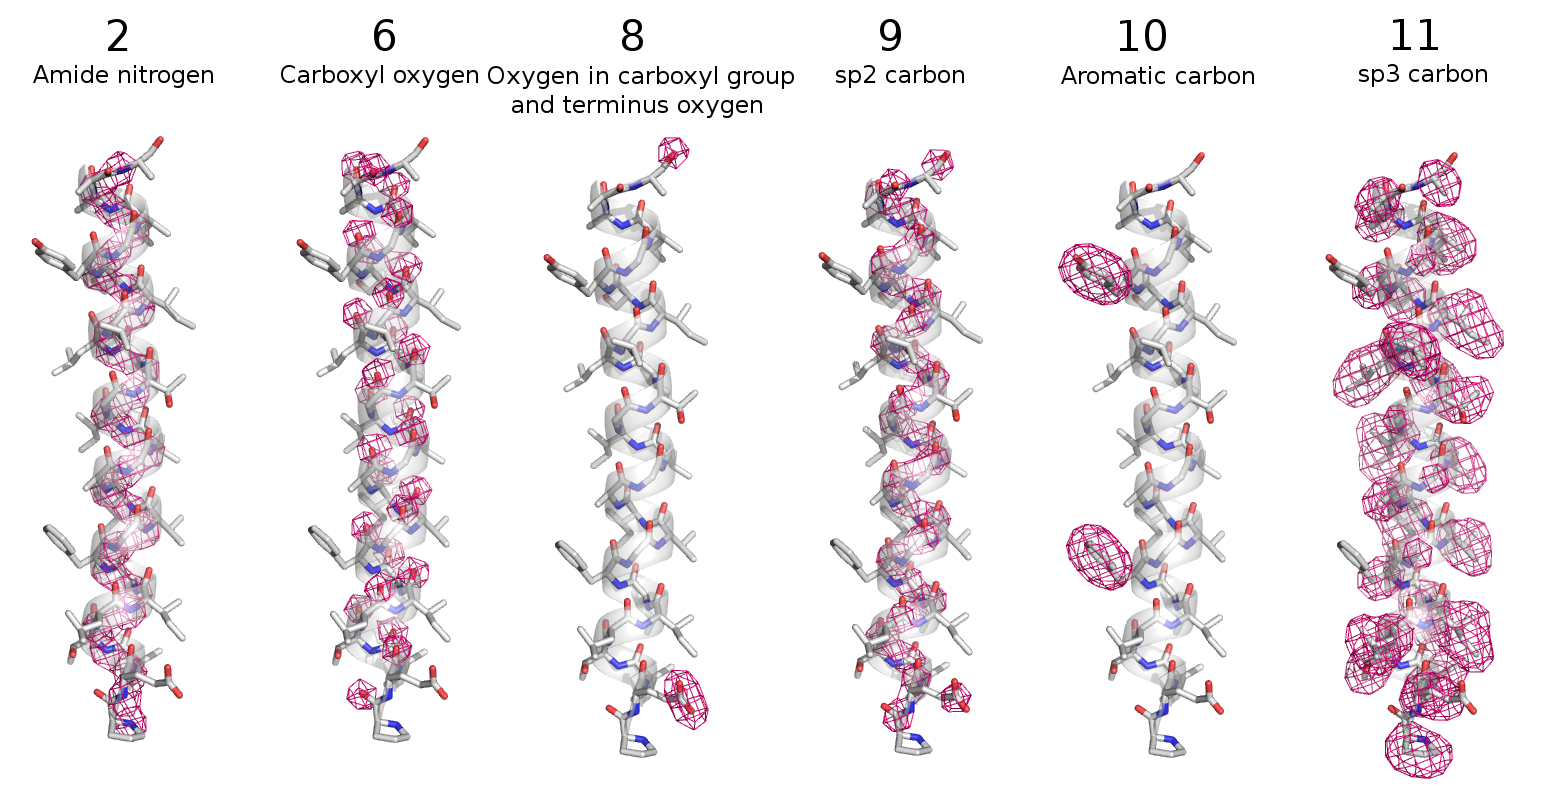
\includegraphics[width=0.7\linewidth]{../draft/Fig/atomic_densities_V3.png}
    \caption{The example of the representation of a protein using atomic densities. The density map is 
    shown using the volumetric rendering plugin for PyMol. The pdb-code of the protein used for this visualization is 5eh6.
    The isosurface level was set to $0.5$.}
    \label{Fig:atomic_densities}
\end{figure}

We use convolutional neural network to predict the quality of a candidate protein structure. The 
schematic representation of the model architecture is presented on the figure below.

\begin{figure}[H]
    \centering
    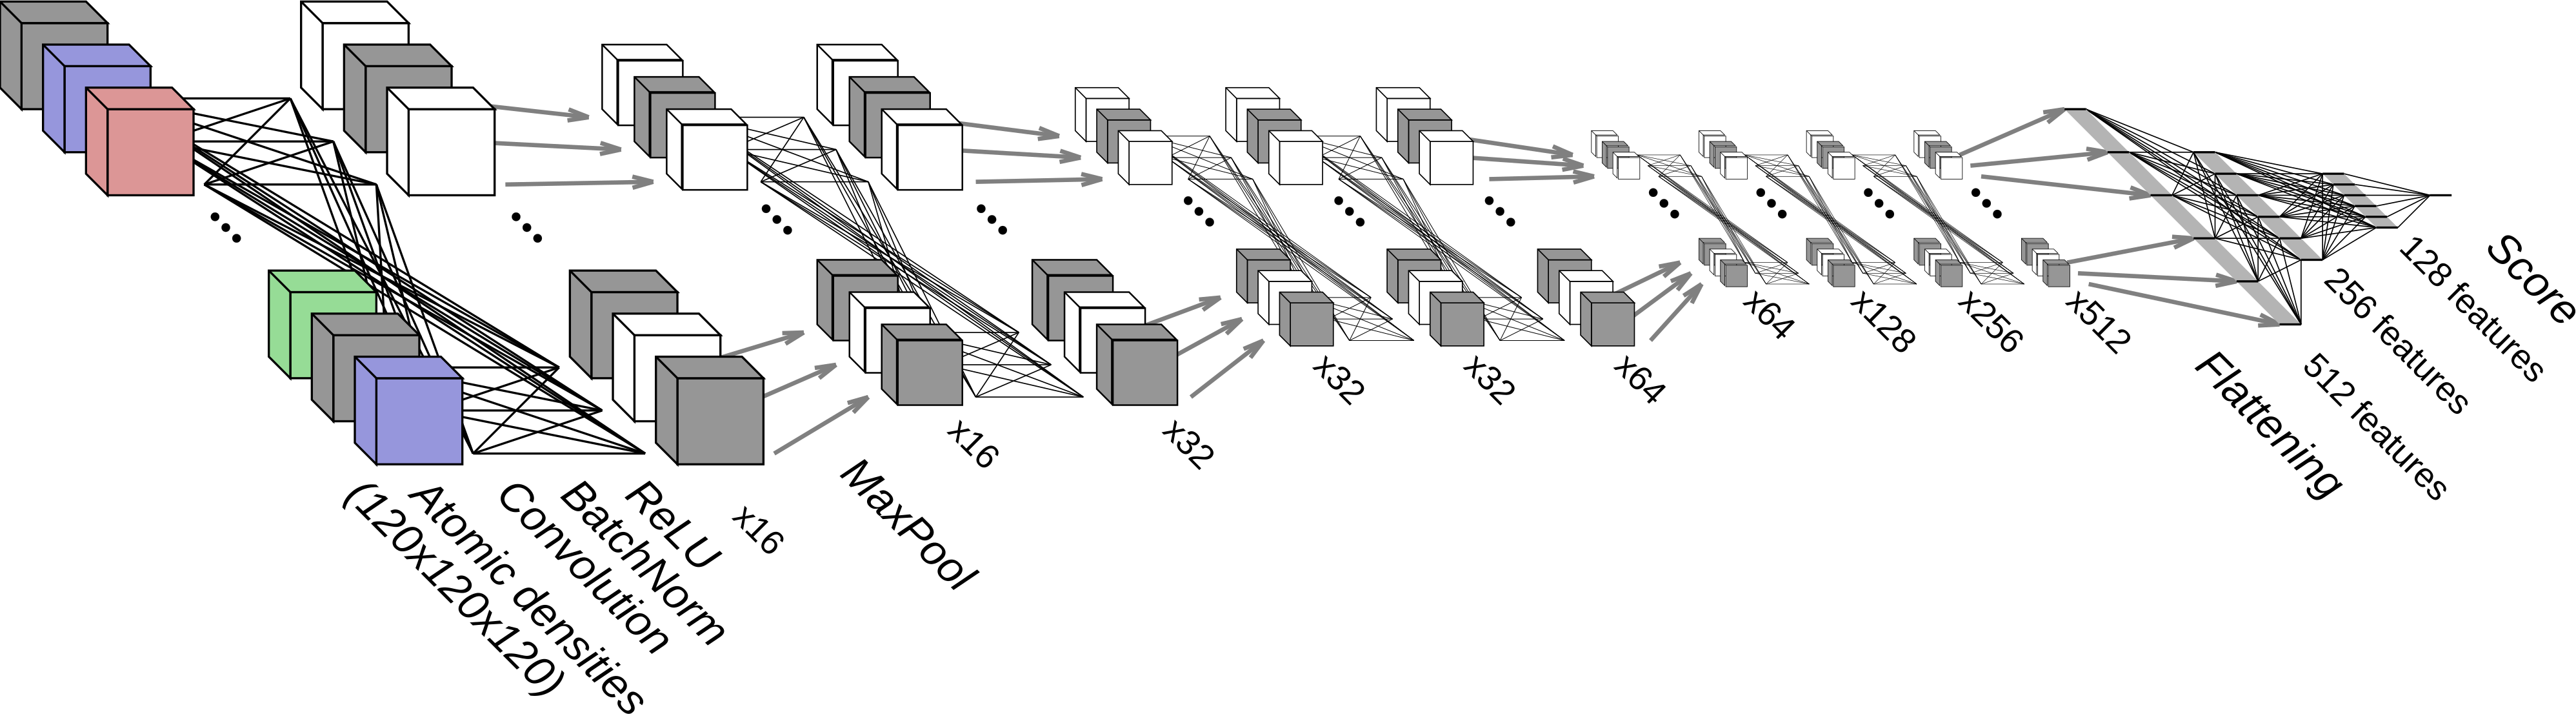
\includegraphics[width=\linewidth]{../draft/Fig/ConvnetDiagramV1.png}
    \caption{The schematic representation of the convolutional neural network architecture used in this work. 
    The arrows between the boxes denote maximum pooling layers and the connections denote 
    consequent 3d convolutional, batch normalization and ReLU layers. The numbers xM denote the number of filters 
    used in the corresponding 3d convolutional layer. The size of all filters and 
    maximum pooling domains are 3x3x3. The grey stripes denote one-dimensional vectors and crossed lines between them 
    stand for fully-connected layer with ReLU non-linearities. The details of the model parameters can be found in 
    Supplementary Information.}
    \label{Fig:CNNModel}
\end{figure}

Finally, the loss function of the model is the pairwise ranking loss:
$$ L_{ij} = w_{ij} \cdot \max \left[ 0, 1 - y_{ij} \left( f \left( x_i \right) - f \left( x_j \right) \right) \right] $$
where $w_{ij}$ is zero when the GDT\_TS of two decoys is too close and one otherwise and $y_{ij}$ is the coefficient that defines the ordering:
$$
y_{ij} = \begin{cases}
               1& gdtts_i \leq gdtts_j \\
               -1& gdtts_i > gdtts_j \\
            \end{cases}
$$
During the training procedure we optimize the loss function with respect to the parameters of the model using stochastic 
gradient descent.

\end{block}

\begin{block}{Datasets}
   To train and assess our method we used the datasets of protein decoys from the CASP competition \cite{moult2014critical}. 
We took the datasets CASP7 - CASP10 as the training set and the CASP11 dataset as the test set.
We optimized side chain conformation of the training and test sets using SCWRL4 program \cite{krivov2009improved}.
The training and test sets have 564 and 83 targets correspondingly. For each target the training dataset has 
on average 282 decoys. The test dataset is split into two subsets: Stage1 with 20 selected decoys for each target and Stage2 with 150 decoys
for each. The native structures were not included in the datasets nor during the training procedure
neither during the testing phase. Fig. \ref{Fig:foldsGraph} shows the overlap between the training and the test sets in terms of 
ECOD structural classification \cite{cheng2014ecod}.
% \begin{figure}[H]
%     \makebox[\textwidth]{
%     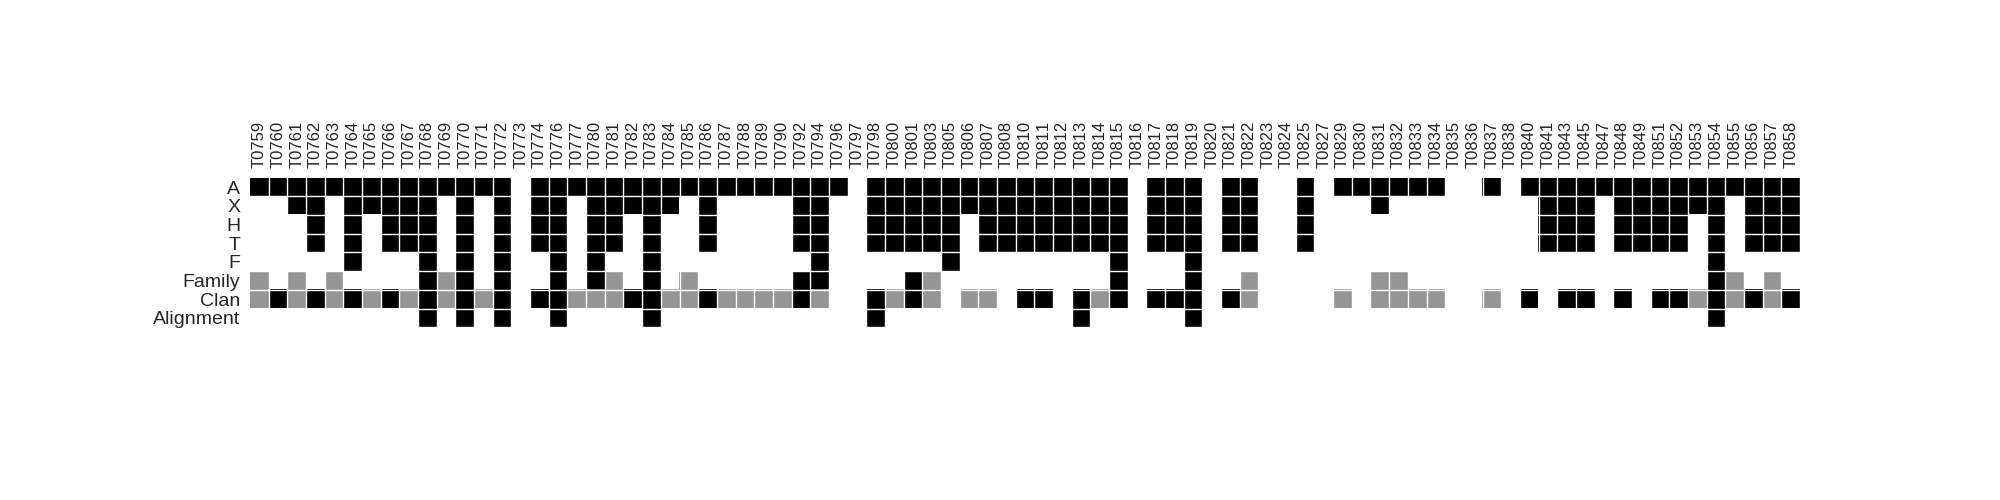
\includegraphics[width=\textwidth]{../draft/Fig/summary_table.png}
%     }
% %
%     \caption{Overlap of the training set on each target domain of the
%     test set (from T0759 to T0858). The first 5 rows of tiles
%     correspond to the ECOD classification of protein domains (A-, X-,
%     H-, T-, and F-groups). A black tile in any of these rows indicates
%     that at least one structure from the training set belongs to the
%     same ECOD group as the target. Targets for which no ECOD
%     classification is available are left empty.
%     A black tile in the ``Family'' row indicates that at least one
%     structure from the training set belongs to the same Pfam family as
%     the target. (A grey tile indicates that no Pfam family information
%     is available for the target.) The ``Clan'' row shows similar
%     information for Pfam clans. A black tile in the ``Alignment'' row
%     indicates that at least one sequence in the training set aligns to
%     the target sequence with an E-value smaller than $10^{-4}$.}
% %
%     \label{Fig:summaryTable}
% \end{figure}
\begin{figure}[H]
    \centering
    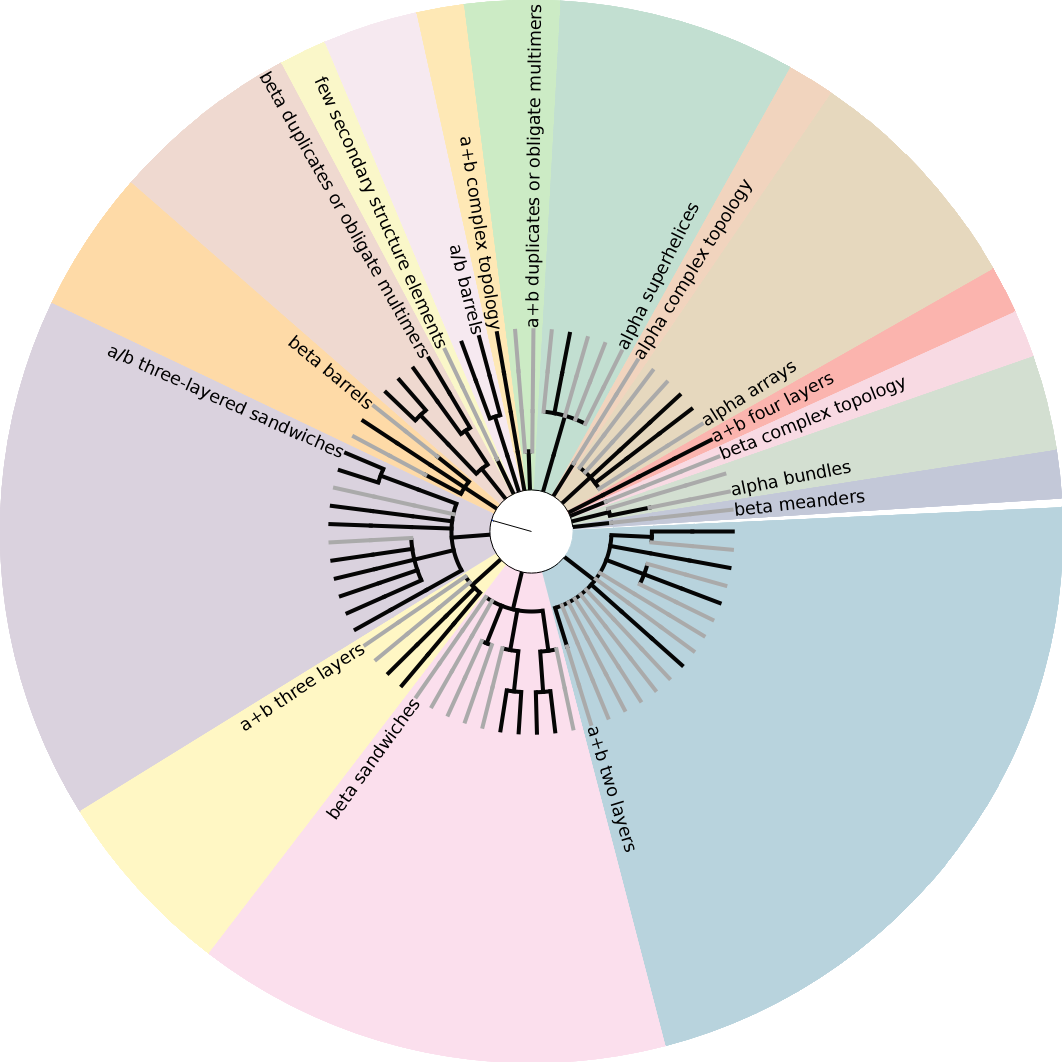
\includegraphics[width=0.6\linewidth]{../draft/Fig/folds_graph.png}
%
    \caption{Classification of the test set structures into the lower
    four ECOD structural levels (from the center out): architecture
    (A), possible homology (X), homology (H), and topology (T). The
    names of the architecture types are shown in the outer circle of
    the diagram.
%%% Why do you have two different architecture names in the same A
%%% group? (brown color: ``alpha complex topology'' and ``alpha
%%% arrays'')
    The grey lines denote test set classes that have no
    respective representative in the training set. The black lines
    show the classes that have representatives in both training and
    test sets. We do not show the F-groups because they have litle
    overlap among the training and test sets.
%%% Why not showing the F-groups?
}
%
    \label{Fig:foldsGraph}
\end{figure}
\end{block}

\end{textblock}


\begin{textblock}{39.0}(43.5,5)

\begin{block}{Results}
To assess the performance of our method (3DCNN) we used different correlation coefficients and the loss.
The loss criterion is the deviation of the GDT-TS of the best decoys for a protein from the GDT-TS score of the decoy with the lowest score:
$$ 
Loss = | max_i( gdtts_i ) - gdtts( argmin(f(x_i) ) |
$$ 

Table \ref{Tbl:TestResults} shows the comparisson of our model with the state of art methods: ProQ2 \cite{ray2012proq2}, 
VoroMQA \cite{olechnovivc2017voromqa}, QProb \cite{cao2016protein} and RWPlus \cite{zhang2010novel} used for the decoy quality assessement. 
To evaluate the performance we used CASP11 stages 1 and 2 datasets.

\begin{table}[H]
\begin{center}
\begin{tabular}{ c | c | c | c | c }
    \multicolumn{5}{ c }{Stage 1} \\ \hline

    QA method & Loss & Pearson & Spearmann & Kendall \\
    \hline
    \textbf{3DCNN}   &0.071 &0.528 &0.414 &0.318 \\
    ProQ2   &0.081 &0.656 &0.534 &0.408 \\
    VoroMQA &0.095 &0.621 &0.504 &0.382 \\
    Qprob   &0.097 &0.631 &0.517 &0.389 \\
    RWplus  &0.128 &0.500 &0.387 &0.291 \\ \hline
    
    \multicolumn{5}{ c }{Stage 2} \\ \hline
    
    ProQ2   &0.058 &0.372 &0.366 &0.256 \\
    \textbf{3DCNN}   &0.067 &0.420 &0.405 &0.285 \\
    Qprob   &0.068 &0.381 &0.387 &0.272 \\
    VoroMQA &0.069 &0.444 &0.437 &0.313 \\ 
    RWplus  &0.095 &0.202 &0.246 &0.175 \\ \hline

\end{tabular}
    
    \caption {Results of our method(3DCNN) and the other state-of-art quality assessment programs on the CASP11 dataset Stage 1 and 2.
            Table shows the absolute average values of the correlation coefficients.}
    \label{Tbl:TestResults}
\end{center}
\end{table}

\end{block}

\begin{block}{Analysis}

During the training of the model we randomly sampled rotational and translational degrees of freedom of a decoy structure. Ideally, we 
want the score assigned by the model to a decoy to be invariant under these transformations. The Fig. \ref{Fig:DecoysScoreDistribution} 
shows the distributions of scores for several decoys.


Figure \ref{Fig:LossVsECOD} shows the performance of the algorithms depending on the presense in the training set of the structures in the same ECOD 
class. We see, that our algorithm has the same performance gains for the proteins 
similar to ones in the test set as the VoroMQA and ProQ2. The algorithm that stands out in this metric is the RWPlus, which 
seems to be indifferent to the homology. However, its performance is also lower than that of the other contenders.

\begin{figure}[H]
    \centering
    \begin{subfigure}{.5\textwidth}
    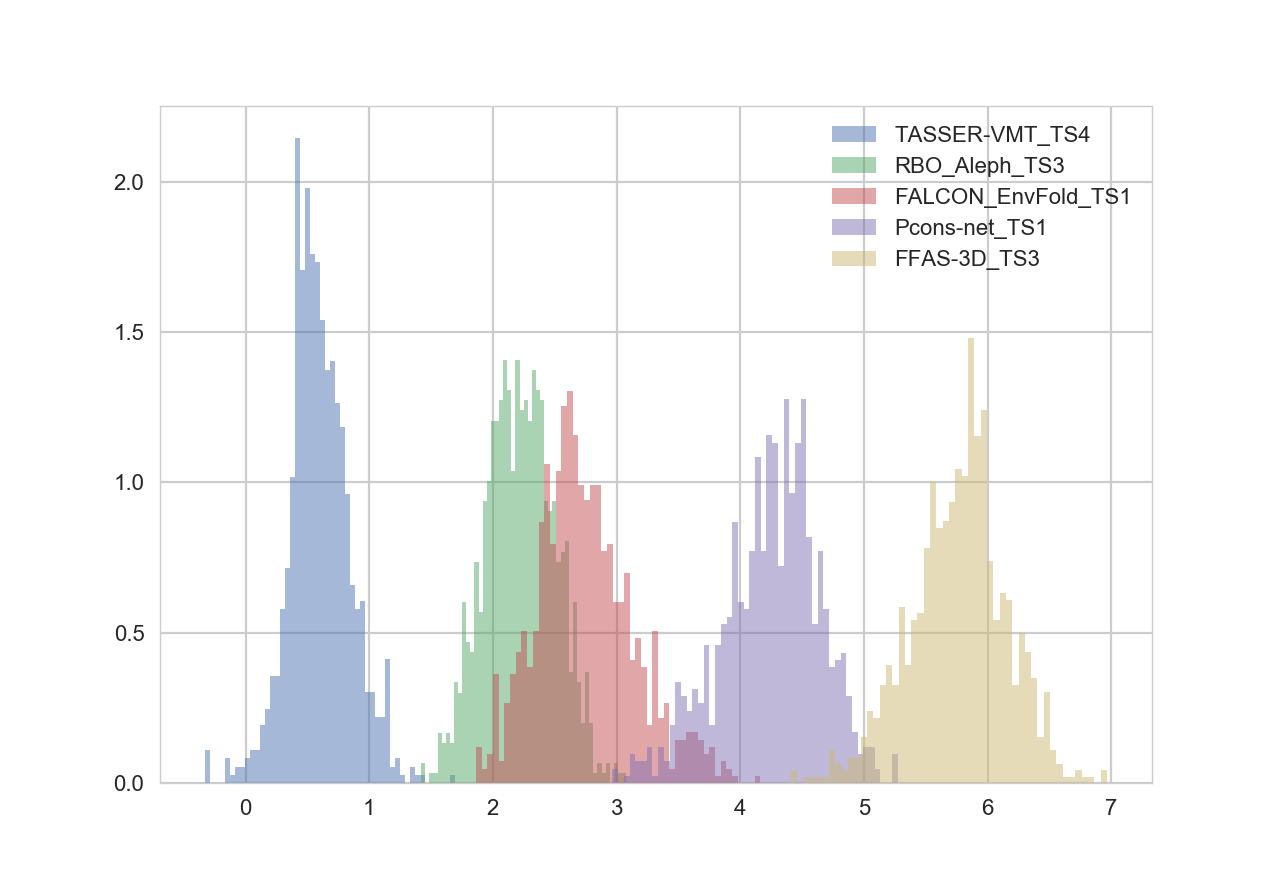
\includegraphics[width=\linewidth]{../draft/Fig/decoys_sampling_dist.png}
    \caption{The distribution of scores under random translations and rotations of several decoys for the target T0832. The 
    names arrangement from top to bottom corresponds to the increase of the score.}
    \label{Fig:DecoysScoreDistribution}
    \end{subfigure}%
    \begin{subfigure}{.5\textwidth}
    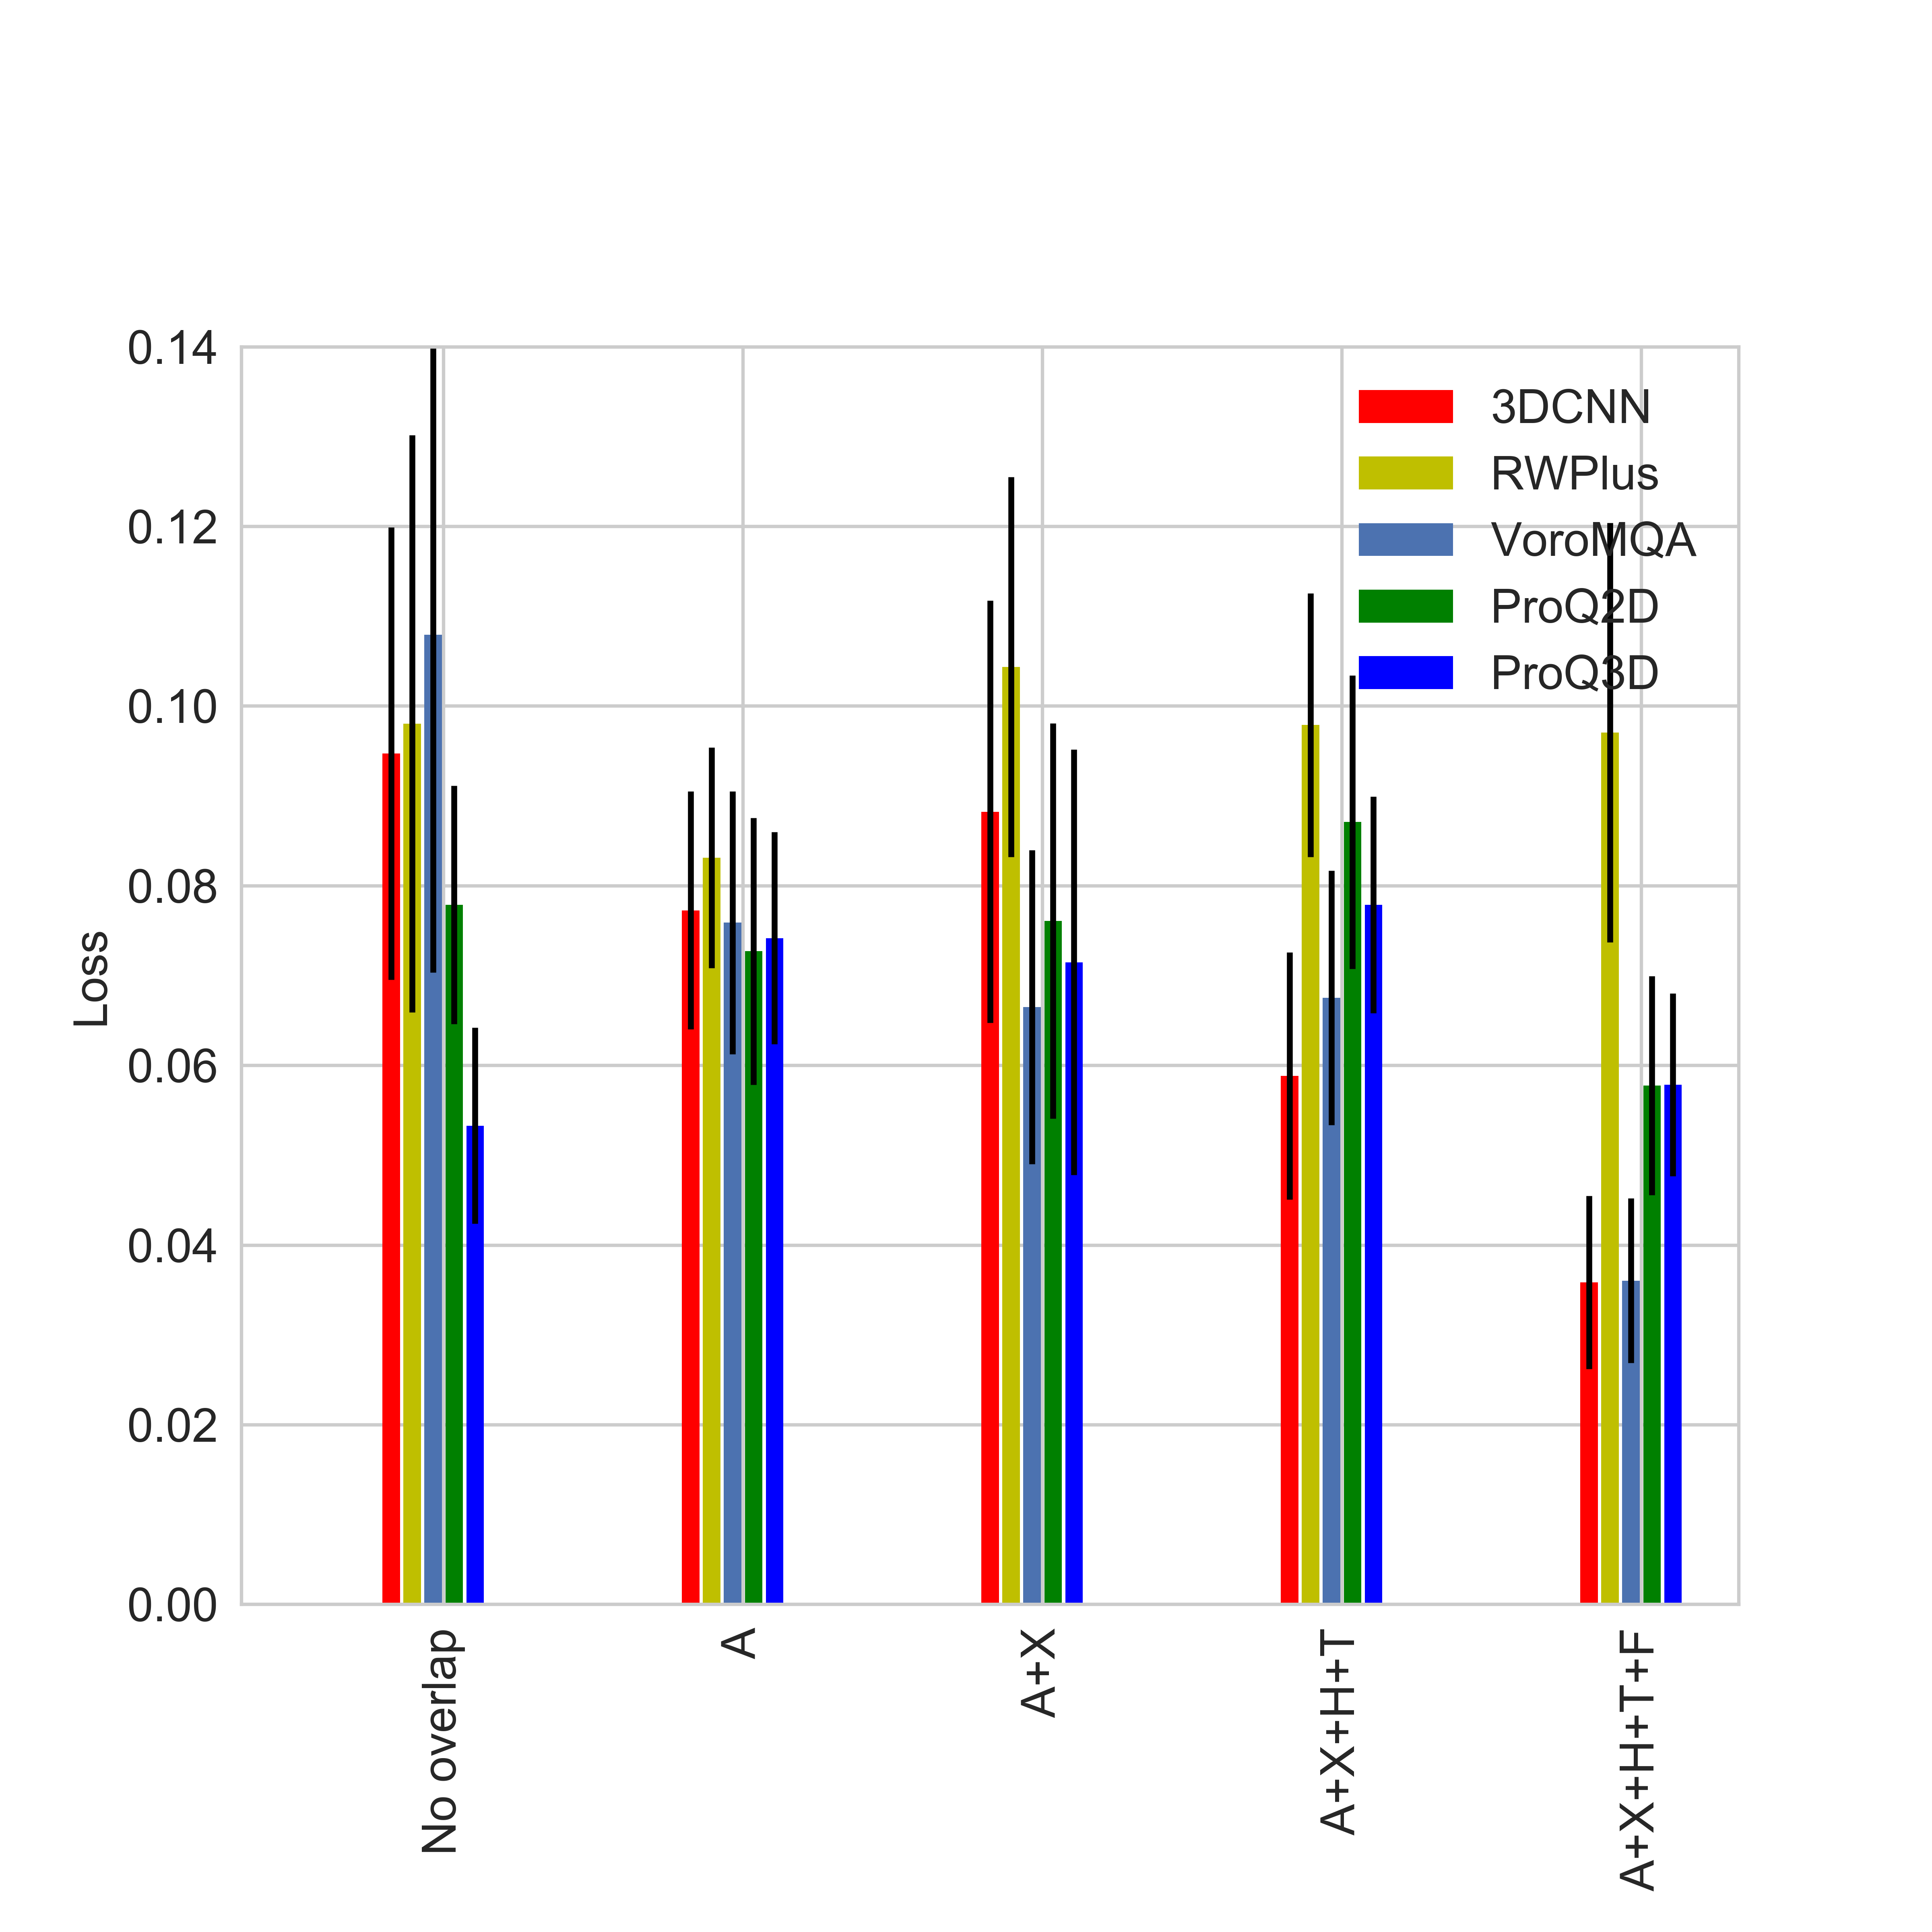
\includegraphics[width=\linewidth]{../draft/Fig/LossVsECOD.png}
    \caption{Loss of different QA-algorithms on the subsets of the CASP11 test set Stage2. The subsets are chosen according to the presense in the
    training set of the structures classified into the same ECOD categories.}
    \label{Fig:LossVsECOD}
    \end{subfigure}
\end{figure}

The method we use was proposed 
by Selvaraju R. \cite{selvaraju2016grad}. The key idea of this technique is to propagate the gradient to a certain layer and take the sum of the 
activations of this layer weighted by gradient. The weighted activation maps are then upscaled to the whole reception field of the network.
They indicate which parts of the input contributes the most to the gradient of the network output. Fig. \ref{Fig:GradCAMT0776_more} shows 
the projection of activation maps obtained using GradCAM on the heavy atoms of a protein.

\begin{figure}[H]
    \centering
    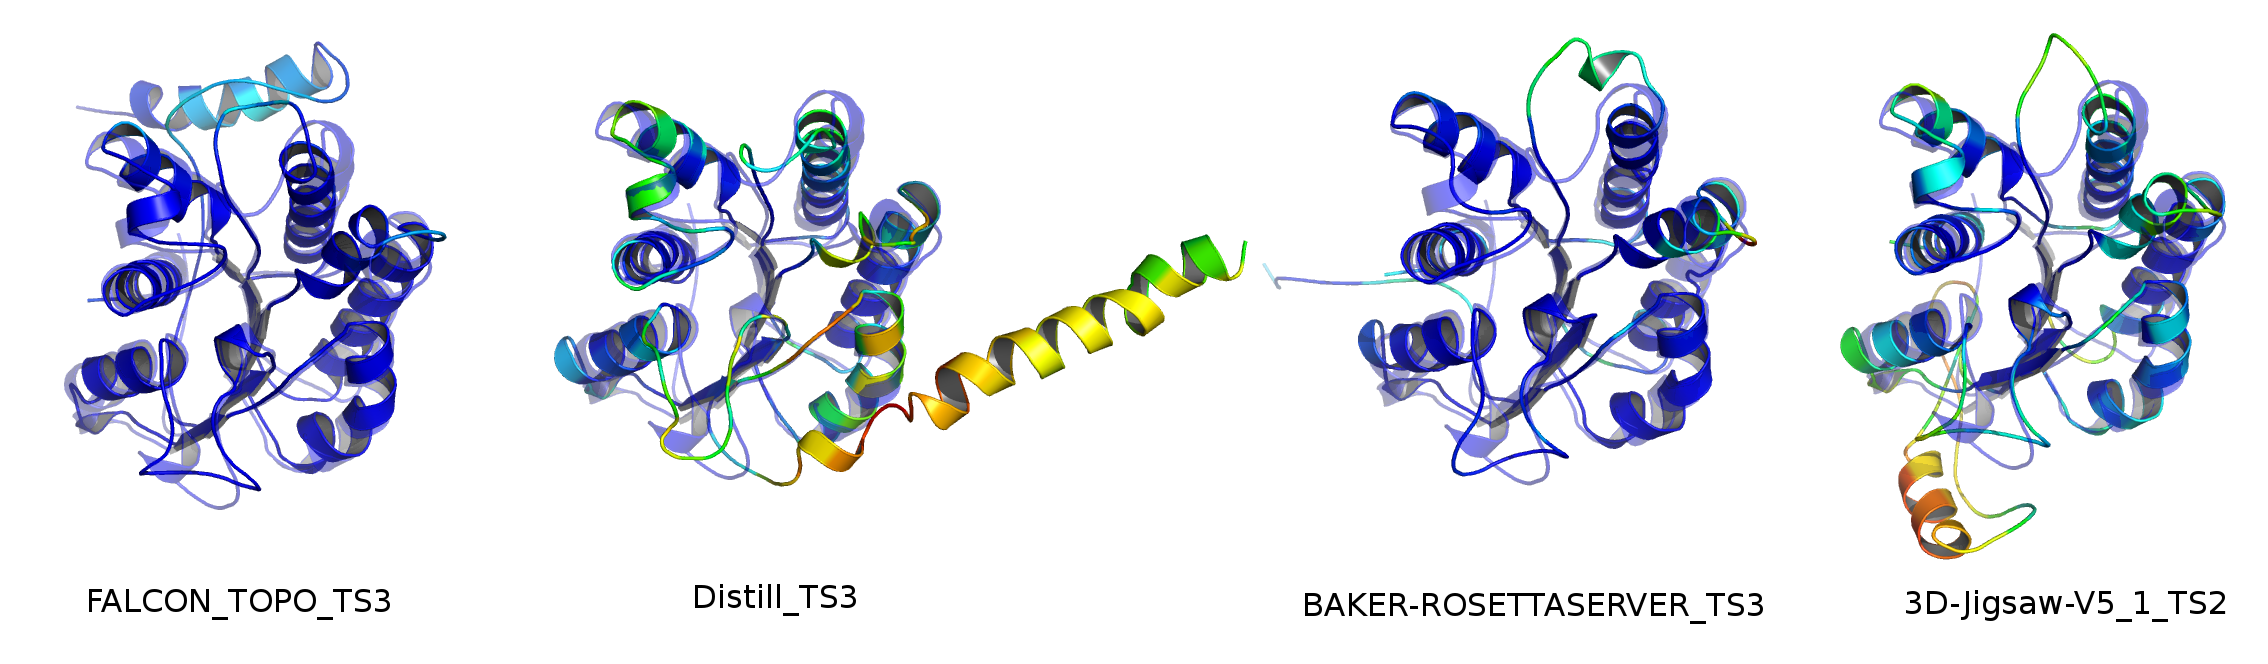
\includegraphics[width=\linewidth]{../draft/Fig/T0776.png}
    \caption{The scaled gradient weighted activation maps of the network projected onto the atoms of the decoys. 
    Each decoy is aligned to the native structure (shown with the transparent cartoon).}
    \label{Fig:GradCAMT0776_more}
\end{figure}
\end{block}


\begin{block}{Citations}
\bibliography{../draft/citations.bib}{}
\bibliographystyle{plain}
\end{block}

\end{textblock}

\end{frame}
\end{document}
